%!TEX root = index.tex
\section[Objetivos]{Objetivos}
\begin{frame}{Objetivos}
\begin{columns}[c] 
\column{.72\textwidth} 

\begin{block}{Sistemas de recomendação}
``São ferramentas e técnicas de software destinadas a prover sugestões de itens para usuários'' \cite{ricci2011introduction-chap1}
\end{block}

\begin{itemize}
	\item \textbf{Biblioteca computacional} para \textbf{sistemas de recomendação}
	\begin{itemize}
		\item Abrangente e adaptável
		\item Leitura de dados e cálculo de sugestões
	\end{itemize}
	\item \textbf{Análise de desempenho}
	\begin{itemize}
		\item Validação cruzada
		\item Precisão e Abrangência 
	\end{itemize}
\end{itemize}


\column{.28\textwidth} 
\begin{figure}[ht]
    \begin{center}
    
\includegraphics[width=0.5\textwidth]{img/r}
    \end{center}
\end{figure}

\begin{figure}[ht]
    \begin{center}
    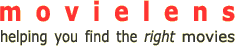
\includegraphics[width=1\textwidth]{img/movielens}
    \end{center}
\end{figure}

\begin{figure}[ht]
    \begin{center}
    \includegraphics[width=1\textwidth]{../img/aws}
    \end{center}
\end{figure}

\end{columns}
\end{frame}
